
% スタイルファイルの指定
% パッケージを使用する場合,ここで全て指定する.
\documentstyle[cite,a4j,twoside,12pt,enumerate,graphicx,listings,amssymb,subcaption,amsmath]{jbmdthesis}
% \documentclass[cite,a4j,twoside,12pt,enumerate,graphicx,listings,amssymb,subcaption,amsmath]{jbmdthesis}

% \usepackage[dvipdfmx]{graphicx}

% ヘッダを追加する
\pagestyle{headings}

% 画像元のパスの追加
\graphicspath{{figure/}}

\begin{document}

% 図,表,節などを参照するためのコマンドを定義
% これらのコマンドの使い方は template/ 内の Readme.md を参照すること
\newcommand{\fig}[1]{{図~\ref{fig:#1}}}
\newcommand{\subfig}[2]{{図~\ref{fig:#1}}~{(\subref{fig:#2})}}
\newcommand{\tab}[1]{{表~\ref{tab:#1}}}
\newcommand{\refchap}[1]{第{\ref{sec:#1}~章}}
\newcommand{\refsec}[1]{{\ref{sec:#1}~節}}
\newcommand{\ctext}[1]{\textcircled{\scriptsize{#1}}}

% ページ番号をアラビア数字にする(0,1,2,..)
\pagenumbering{roman}


% ---------- ユーザ入力ここから ----------
% タイトルページの情報
\title{\bf 容量効率を意識したソース・タグ値に \\
基づくセグメント化による\\
発行キューの電力削減}
\author{\bf 森 健一郎}
\date{3} % 令和~年

% 表紙を出力(自分の所属に応じてコメントを外す)
\minfotitle   % 修論
% \belectitle   % 卒論
% ---------- ユーザ入力ここまで ----------



% 概要を出力
{ 
  % 目次に影響がでないように, 
  % setlength のスコープを abstract 内だけに限定するためのブロック

  % 行間の調整
  \setlength{\baselineskip}{2.2em}
  
\chapter*{概要}
\markboth{概要}{概要}
近年のサーバー・アプリケーションや,JavaScriptで書かれたWebアプリケーションでは,従来のアプリケーションと比べて命令キャッシュ・ミスが特に多く発生することが知られている.これに対し,命令キャッシュ向けのプリフェッチャが多く研究されており,非常に高いキャッシュ・ヒット率が達成されている.しかし,それらのプリフェッチャでは高い性能をもつものほど大きな追加資源が必要になる.例えば,最先端の命令プリフェッチャであるProactive Instruction Fetchでは,L1命令キャッシュそのものより大きなテーブルを必要とする.また,プリフェッチのミスに対するカバー率こそ高いものの,無駄なプリフェッチを多く実行してしまい,電力を無駄に消費してしまう場合がある.

これに対し,本論文では命令プリフェッチのアプローチではなく,フェッチ・ステージのパイプライン構造の工夫によりフェッチ・スループットを向上させる手法を提案する.本提案手法はプリフェッチャと異なり,複雑な機構や大きなテーブルも必要なく,無駄なメモリアクセスを全く行わない.さらに,性能低下のデメリットなしに命令キャッシュ・ミスによるストールを削減し,フェッチ・スループットを向上させることができる.
提案手法をサーバー向けのベンチマークを用いて評価したところ,プリフェッチを行わない場合と比較して最大 25.8\%,平均で13.0\%の性能向上を達成した.また,最先端の命令プリフェッチャと比較して平均4.8\%の性能向上が得られることを確認した.

}

% 目次を出力
\tableofcontents

% ページ番号のリセット
\clearpage 
\pagenumbering{arabic}

% 行間の調整(これ以降ずっとこの行間)
\setlength{\baselineskip}{2.2em}



% ---------- ユーザ入力ここから ----------
% 各章の記述

\chapter{はじめに}
\label{sec:introduction}
近年のプロセッサは,命令キャッシュ・ミスによる性能低下が問題となっている.これは,現代のアプリケーションの命令ワーキング・セットが大きくなっていることに由来する.このようなアプリケーションの例として,オンライントランザクション処理などのサーバー向けのアプリケーション~\cite{Ranganathan1998,Vaidya2008,Ferdman2012}や,JavaScriptを用いたWebアプリケーション~\cite{Zhu2015,Chadha2014},クラウドのアプリケーション~\cite{Ferdman2012,Ayers2019}がある.これらのアプリケーションは,命令フットプリントが膨大であり,L1命令キャッシュに収まらないため,命令キャッシュ・ミスが多く発生する.命令キャッシュ・ミスが発生すると,プロセッサに実行できる命令を供給できなくなるため,それにより性能が低下する.これは近年の高性能なアウト・オブ・オーダー実行方式のプロセッサにおいても命令キャッシュ・ミスにおけるストールは隠蔽することが難しいため,重要な問題である.

この問題に対し,命令キャッシュ・ミスを減らす手法として,命令プリフェッチャがある.命令プリフェッチャは,ある命令が要求される前に,その要求を先読みして下位レベルのメモリへアクセスを行い,あらかじめその命令をキャッシュへと転送する.これを命令プリフェッチという.命令プリフェッチが成功すると,命令キャッシュ・ミスを回避できるため,性能低下を抑えることができる.

命令プリフェッチャには様々なものが提案されている.例えば,単純なものとしてミスしたラインの次のラインをプリフェッチするネクストライン・プリフェッチャがある.また,分岐予測器が持つ情報を使用するFetch Directed Instruction Prefetching~\cite{Reinman1999}や,命令キャッシュ・ミスのストリームを記録して命令プリフェッチを行うTemporal Instruction Fetch Streaming~\cite{Ferdman2008},及びそれを改良した非常に高いプリフェッチ効果をもつProactive Instruction Fetch (PIF)~\cite{Ferdman2011}などが提案されている.

しかし,これらのプリフェッチャは,性能が高いものほど非常に大きなコストが必要になる.なぜなら,有効なプリフェッチを行うためには,複雑なキャッシュ・ミス・パターンを予測するアルゴリズムをハードウェアで実現する必要があるからである.特にPIFは,命令キャッシュ・ミスを90\%以上削減することが可能であるが,必要なストレージのサイズは一般的なL1命令キャッシュよりも非常に大きい(L1命令キャッシュが32KBに対し,200KB程度).さらに,このようなプリフェッチャは,プリフェッチのミスに対するカバー率こそ高いものの,無駄なプリフェッチを実行することもあり,その分電力を余分に消費してしまう.

そこで,本論文では命令プリフェッチのアプローチではなく,命令フェッチ部のパイプライン構造を工夫することによって命令フェッチのスループットを向上させる以下のような手法を提案する.
\begin{enumerate}
  \item 従来の命令フェッチ・パイプラインでは,L1命令キャッシュがヒットすることを前提としてパイプラインが設計されており,命令がフェッチされるとその命令は直ちに次のステージが送られる.これに対し,本研究ではMiss-assuming Pipeline (MAP) と呼ばれる新しいパイプライン構造を提案する.MAP は L1 命令キャッシュのミスを前提としてパイプラインが設計されており,命令キャッシュがヒットしてもミスしても常に一定のレイテンシでフェッチを行う.この動作により,MAP では命令キャッシュ・ミスが発生してもフェッチのスループットを損なうことなく,実行を継続できる.
  \item しかし,MAP は従来のパイプラインと比べてパイプライン段数が増加なるため,分岐予測ミス・ペナルティが増加してしまう.MAPの 利点を最大限活用しつつこの欠点に対処するために,本研究ではフェッチのパイプライン構造を,従来のパイプラインと MAP の間で動的に切り替えて使用するアーキテクチャを提案する.同時に,本論文ではこのアーキテクチャによって得られる恩恵を最大化するための最適なパイプラインの切り替えアルゴリズムを提案する.このアルゴリズムを用いると,MAP による分岐予測ミス・ペナルティ増加の影響を最小にすることができ,得られる恩恵を最大化することができる.
\end{enumerate}

提案手法は,プリフェッチャとは異なり無駄なメモリ・アクセスを全く行わない.また,従来のプリフェッチャのような複雑な機構や大きなテーブルも必要なく,非常に低コストで構成することができる.さらに,本提案手法を適用すると,性能低下のデメリットなしに命令キャッシュ・ミスによるストールを削減でき,命令キャッシュ・ミスが多く発生するような状況においては,大きな性能向上が期待できる.

本論文の構成は次の通りである.まず,\refchap{related_work}で関連研究を示す.\refchap{miss_assumed_pipeline}では MAP について説明する.その後,\refchap{hybrid_arc}で従来の構成と MAP を組み合わせたアーキテクチャについて述べ,\refchap{sw_algorithm}では提案するパイプラインの切り替えアルゴリズムについて述べる.\refchap{evaluation}では提案手法の評価を行い,最後に\refchap{summary}でまとめる.



\chapter{発行キュー(IQ:Issue Queue)}
\label{sec:basic_IQ}
本章では,本研究の研究対象である,IQ に関して説明する.まず,IQ の概要と動作を\refsec{iq_abst}で説明したあと,IQ の回路構成を\refsec{iq_circuit}で述べる.その後,\refsec{iq_scheme}でIQ の方式に関して説明する.

\section{概要と動作}
\label{sec:iq_abst}
IQ はアウト・オブ・オーダ実行のプロセッサにおいて,リネームされた命令を保持し,実行順序をスケジューリングして,機能ユニットへ発行する回路である.IQ は,ディスパッチ,発行,ウェイクアップと呼ばれる 3 種類の動作を行う.以下でそれぞれの動作に関して説明する.

\begin{itemize}
  \item ディスパッチ:リネームされた命令は,IQ にエントリが割り当てられ,命令の情報が格納される.この動作をディスパッチと呼ぶ.ディスパッチの動作は,IQ の方式により異なる.IQ の方式に関しては,\refsec{iq_scheme}で詳しく説明する.
  \item 発行:IQ 内の命令のうち,ソース・オペランドが両方共レディとなった命令は,依存関係が解消し,実行が可能となる.このような命令を実行ユニットに送出する動作を発行と呼ぶ.なお,発行可能な命令が機能ユニットの数を超える場合は,各命令の発行優先度に基づき命令を選択して発行する.発行された命令のエントリは IQ より削除される. 
  \item ウェイクアップ:命令が発行されると,その命令のデスティネーション・オペランドのタグと IQ 内にある全命令のソース・オペランドのタグの比較が行われる.比較が一致した場合には,対応するソース・オペランドのレディ・ビットをセットする.この動作をウェイクアップと呼ぶ.両方のオペランドがレディとなった命令は,依存が解消したため発行可能となる.
\end{itemize}

\begin{figure}[htb]
  \centering
  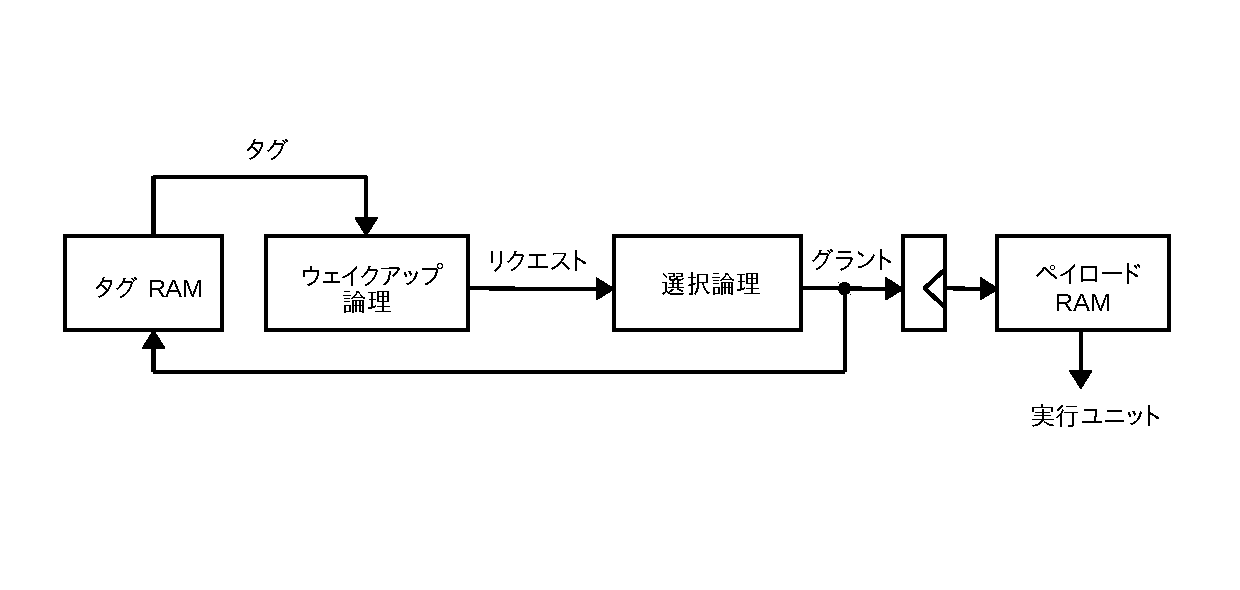
\includegraphics[keepaspectratio, scale=.8]{iq_logic}
  \caption{IQ の回路構成}
  \label{fig:iq_logic}
\end{figure}

\section{回路構成}
\label{sec:iq_circuit}
\fig{iq_logic}に IQ の回路構成を示す.IQ はウェイクアップ論理,選択論理,タグ RAM,ペイロード RAM と呼ばれる 4 つの回路より構成される.以下で各回路に関して説明する.また,IQ の回路のうちウェイクアップ論理は提案手法に関わる重要な回路であるため,\refsec{wakeup_logic}にて詳細に説明する.

\begin{itemize}
  \item ウェイクアップ論理:命令間の依存関係を管理し,他の命令との依存関係が解消された命令について発行要求(リクエスト信号)を出す.
  \item 選択論理:資源制約を考慮して,発行を要求された命令の中からそれを許可する命令を選択し,発行許可信号(グラント信号)を出力する.この選択においては,回路の単純化のために IQ の先頭のエントリの命令をより優先する.
  \item タグ RAM:発行待機中の命令のデスティネーション・タグを保持する回路で,選択論理から発行許可信号が送られると,対応する命令のタグが読み出され,ウェイクアップ論理へ送られる.
  \item ペイロード RAM:発行待機中の命令のコードを保持する.選択論理から発行許可信号が送られると,対応する命令のコードを実行ユニットに送出する. 
\end{itemize}

\subsection{ウェイクアップ論理}
\label{sec:wakeup_logic}
\fig{wakeup_logic}に,ウェイクアップ論理の回路を示す.図中の $IW$ は発行幅を,$IQS$ は IQ のエントリ数を表す.ウェイクアップ論理では,$IW$ 個のデスティネーション・タグ(dtag)が IQ 内の全命令に放送される.各命令は 2 つのソース・タグ(stag)を保持しており,放送されたデスティネーション・タグと比較される.いずれかのデスティネーション・タグとソース・タグが一致した場合,そのソース・オペランドのレディ・ビットがセットされる.2 つのレディ・ビットがセットされた命令は発行が可能となるため発行要求が出力される.

\fig{cam}に,IQ に使用されるタグ比較器の CAM 回路を示す.同図は,ソース・タグ 1 ビット分の比較回路を表す.同図に示すように,高速化のため通常ダイナミック論理によって構成される~\cite{Palacharla1997}.比較の動作は,次のように行われる.まず,マッチ線がプリチャージされる.次にデスティネーション・タグが放送され,比較が行われる.タグが不一致であれば,直列に接続された 2 つのプルダウン・トランジスタが両方とも ON となり,マッチ線がディスチャージされる.タグが一致する場合,マッチ線は $H$ の状態が維持される.比較器はマッチ線のディスチャージ時に電力を消費する.

\begin{figure}[htb]
  \centering
  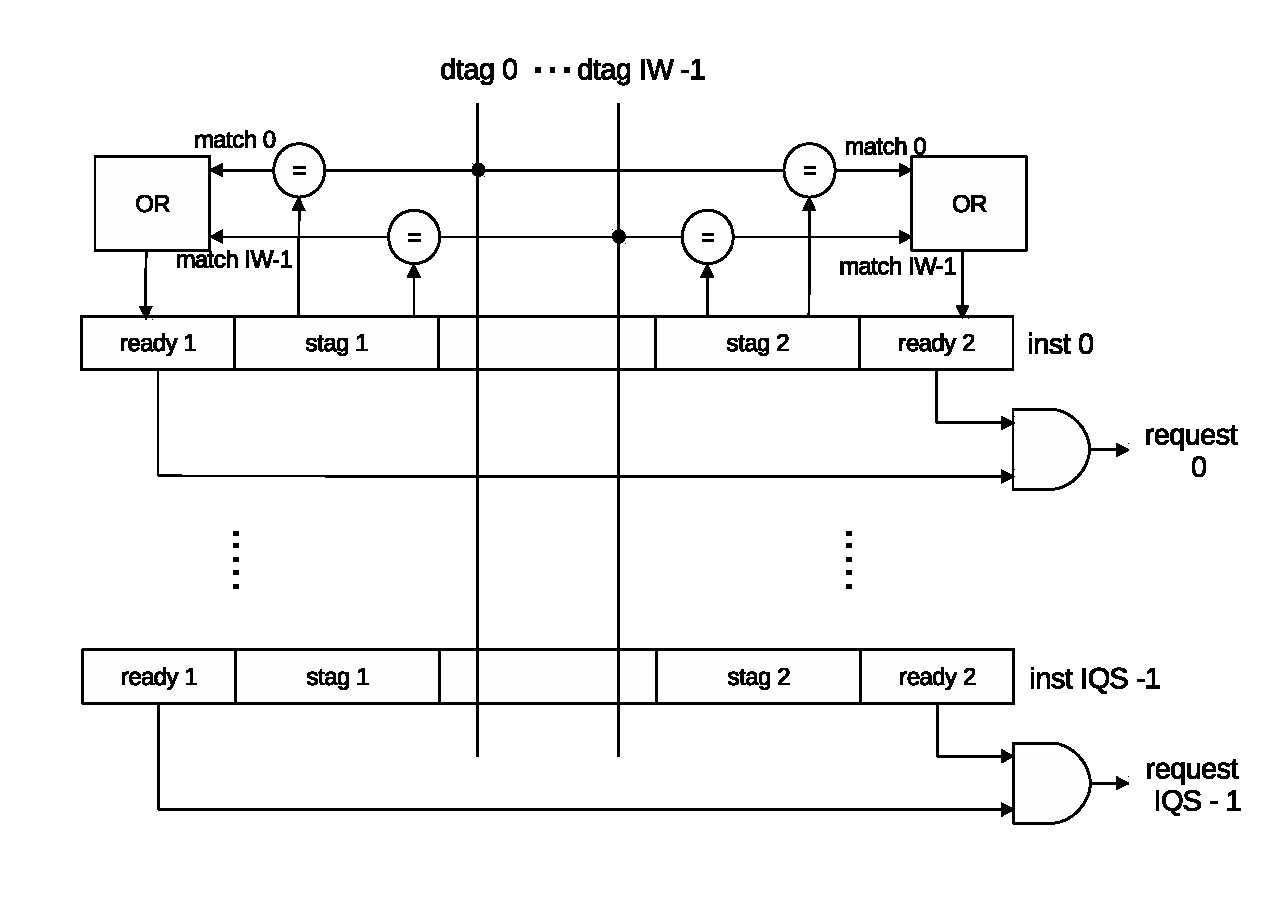
\includegraphics[keepaspectratio, scale=.8]{wakeup_logic}
  \caption{ウェイクアップ論理}
  \label{fig:wakeup_logic}
\end{figure}

\begin{figure}[htb]
  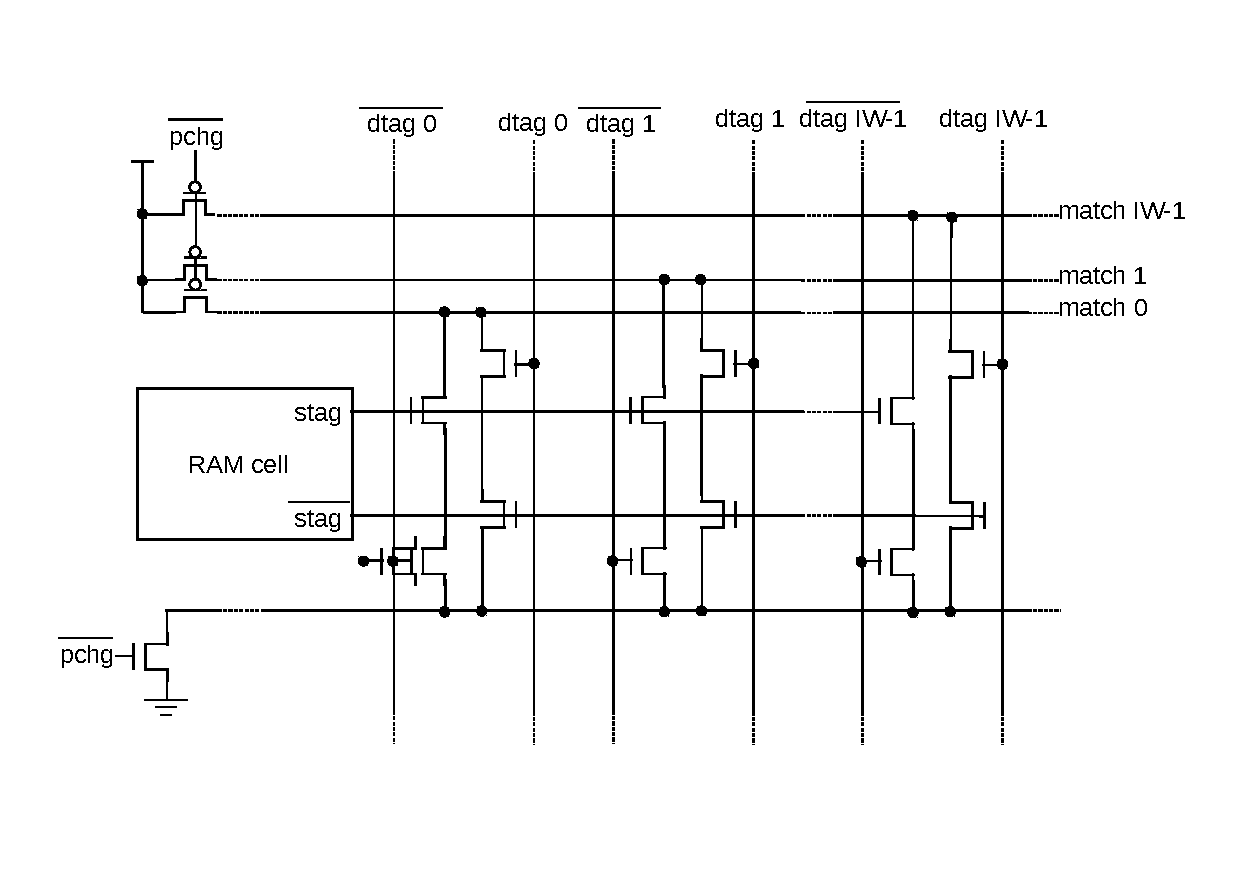
\includegraphics[keepaspectratio, scale=.8]{cam}
  \caption{タグ比較器の CAM 回路}
  \label{fig:cam}
\end{figure}

\section{IQ の方式}
\label{sec:iq_scheme}
これまで,IQ の方式としてシフト・キュー,サーキュラ・キュー,ランダム・キューの 3 つの方式が商用プロセッサで使用された.各方式に関して説明した後,現在主流の方式であるエイジ論理付きのランダム・キューに関して説明する.

\subsection{シフト・キュー}
シフト・キューは,非常に古い(20 年以上前)商用プロセッサに使用された IQ の方式である~\cite{Farrell1998}.シフト・キューでは,IQ は基本的に FIFO バッファであり,末尾のエントリに命令をディスパッチする.これにより,古い命令に高い発行優先度を与えることができる.\footnote{一般に,古い命令から優先的に発行すると,性能がより高くなることが知られている~\cite{Butler1992}.}

また,シフト・キューでは命令を発行したエントリの空きを詰めるコンパクションを行うことにより,高い容量効率も達成することができる.正しい発行優先度と,高い容量効率を同時に達成するため,シフト・キューは IQ の方式の中で最も高い性能を得ることができる.

一方でシフト・キューには,コンパクションの回路が非常に複雑で,また消費電力が非常に大きいという欠点がある.そのため,シフト・キューはスケーリングが困難であり,現在のプロセッサでは使用されていない.

\subsection{サーキュラー・キュー}
サーキュラー・キューは,シフト・キューと同様,命令をプログラム順に並べるが,コンパクションを行わない方式である~\cite{Abella:survey2003}.サーキュラー・バッファで実装される.

サーキュラー・キューでは,先頭と末尾の間の命令が発行されても,新たに命令をディスパッチできないため,IQ の容量効率がシフト・キューと比較して低下する.また,ヘッド・ポインタとテール・ポインタの位置が逆転するラップ・アラウンドが生じた際には,新しい命令に高い優先度が与えられる優先度逆転が起き,選択論理が正しい優先度で命令を選択できない.これらの理由から,サーキュラー・キューはシフト・キューと比較して性能が低下する.特に,容量効率が低下する影響は大きく,現在のプロセッサでは使用されていない.

\subsection{ランダム・キュー}
近年は,回路の単純化や電力削減のため空いているエントリに単純にディスパッチするランダム・キューが使用されている~\cite{Alpha21464, AMD-Bulldozer, IBM-Power8}.ランダム・キューでは IQ の容量を無駄にすることがなく,高い容量効率を達成する.その一方で,命令が年齢とは無関係にランダムに並ぶため,正しい優先度で命令を発行することができない.

ランダム・キューでは,IQ の空きエントリのインデクスを保持するフリー・リストを用意する.ディスパッチ時には,フリー・リストから読み出したインデクスが指す IQ のエントリに命令を書き込む.IQ から命令が発行されエントリが無効化されると,そのインデクスをフリー・リストへ返す.フリー・リストは FIFO バッファで管理される.

\subsection{エイジ論理付きランダム・キュー}
ランダム・キューにおける発行優先度に関する欠点を緩和するため,ランダム・キューは一般にエイジ論理が併用される~\cite{Alpha21464}.エイジ論理は選択論理と並列に動作する回路で,発行要求が出された命令の中で最も古い 1 命令を選ぶ.最も古い命令はクリティカル・パス上の命令である可能性が高いため,これを優先して発行することができ,結果としてエイジ論理付きランダム・キューは通常のランダム・キューと比較して性能が大きく向上する.

本研究における IQ は,エイジ論理付きのランダム・キューを仮定する.




\chapter{関連研究}
\label{sec:related_work}
本章では,IQ に関連する研究について述べる.\refsec{relate_IQ}で IQ に関する一般的な関連研究に関して説明し,\refsec{relate_IQ} で IQ の研究のうち,電力に関係する研究を述べる.

\section{IQ に関する関連研究}
\label{sec:relate_IQ}
Palacharlaらは,命令発行幅とIQのサイズを変化させた時の,ウェイクアップ論理と選択論理の遅延を評価した~\cite{Palacharla1997}.また,遅延を小さくするために,IQを複数のFIFOバッファで構成し,依存する命令を同じFIFOバッファに割り当てる依存ベースのIQを提案した.この手法では,各バッファの先頭の命令のみ発行可能かチェックすれば良いので,回路が単純化され遅延が減少する.

Starkらは,IPCをほとんど低下させずに,ウェイクアップ論理と選択論理をパイ
プライン化する手法を提案した\cite{Stark2000}.この手法では,投機的にウェイクアップを行うことで,依存する命令を連続するサイクルで発行できるようにした.

五島らは,ウェイクアップ論理を従来のCAMではなく,依存行列と呼ぶRAMで構成する手法を提案した\cite{goshima2001}.これによって比較器を用いずに依存する命令をウェイクアップすることが可能で,ウェイクアップの遅延を短縮できる.

Sassoneらは,依存行列の遅延と電力をより小さくするための手法を提案した\cite{sassone2007}.具体的には,従来はすべての命令について,その古さを完全に追跡していたのに対して,命令をグループ化してグループ単位で古いものを選択する.これにより,性能低下を最小限に抑えながら,回路の規模を小さくできる.

Lebeckらは.キャッシュ・ミスするロードのような長いレイテンシの命令に依存する命令を,IQとは別の待機用バッファに入れ,その長いレイテンシの処理が完了するまでIQに挿入しないという方式を提案した\cite{Lebeck2002}.これによって,IQが待機する命令で埋ることによって起こるストールの頻度が減り,性能が向上する.

Raaschらは,IQをいくつかのセグメントに分割する方式を提案した\cite{Raasch2002}.この方式では,各命令の依存命令チェーンのレイテンシを元に割り当てるセグメントが決定される.そして,発行可能になる直前に最下位セグメントである発行バッファに命令を移動する.この発行バッファでのみ発行を行うことで,すべてのエントリから発行できる通常のIQと比較して遅延を短縮できる.

Kimらは,レイテンシが互いに1サイクルの依存関係のある2つの命令をグループ化し,1つの命令としてIQのエントリでスケジューリングすることで,依存グラフのエッジのレイテンシ短縮とキューの容量効率を上げる手法を提案した\cite{Kim2003}.

Gibsonらは,依存する命令をポインタでつなぎ,ポインタをたどることでウェイクアップを行う手法を提案した\cite{Gibson2010}.この方式によりCAMが不要になり,電力を削減できる.

安藤らは,実行プログラムの命令レベル並列性(ILP)とメモリ・レベル並列性(MLP)に応じて IQ の方式を切り替える手法を実装した\cite{Ando2019}.ILP と MLP のいずれかが高い場合は IQ の容量効率が重要であるため,ランダム・キューで実行する.ILP も MLP もいずれも低い場合には,容量効率よりも正しい発行優先度のほうが重要であるためサーキュラー・キューで実行する.

甲良らは,実行プログラムの ILP と MLP に応じて IQ のサイズを変化させる手法を提案した\cite{Kora2013}.本手法では,いずれかが高い場合には,IQ の容量が重要となるため IQ のエントリ数を増加し,どちらも低い場合には IQ のエントリ数を減少させる.

\section{IQ の電力削減に関する関連研究}
\label{sec:relate_energy}
Folegnaniらは,空のエントリの比較器や既にレディなオペランドを持つ比較器など,タグを比較する必要がない比較器を動作させないことで,消費エネルギーを削減する手法を提案した\cite{folegnani2001}.

Ponomarev らは,リソース要求に応じて 発行キューのサイズをリサイズすることにより,消費エネルギーを削減する手法を提案した~\cite{ponomarev2001} .

Ernstらは,IQに入ってくる命令のうちのほとんどが,はじめから少なくとも1つのソース・オペランドがレディであると指摘した\cite{ernst2002}.そしてIQに,2つのソース・オペランドを保持できるエントリに加えて,1つのソース・オペランドのみ保持できるエントリと,ソース・オペランドを保持しないエントリを用意し,レディでないソース・オペランドの数に応じていずれかにディスパッチする手法を提案した.さらにこの手法を実現するために,命令の2つのオペランドの内,あとにレディになるオペランドを予測する手法である Last Tag Prediction も提案した.

Sembrant らは,クリティカル・パス上にない命令を発行キューとは別のバッファに入れ,ディスパッチを遅延させることによって,性能を低下させずに発行キューのサイズを小さくする手法を提案した~\cite{Sembrant2015}.

Homayoun らは,キャッシュ・ミスの処理中に発行幅を半減させることで,IQの消費電力を削減する手法を提案した\cite{H.Homayoun2011}.発行幅半減中に元の発行幅の半分以上の命令が発行される場合,一時的にその命令を小さなバッファに移動させることで対応している.

松田らはウェイクアップ時のタグ比較を 2 段階に分割することによりエネルギー削減を行う方法を提案した\cite{kobayashi-thesis, matsuda-thesis}.この方法では,タグの比較を高位ビットと低位ビットに分割し,低位ビットの比較を最初のサイクルで行う.そして低ビットが一致していた場合のみ,次のサイクルで高位ビットの比較を行うことによってエネルギーを削減する.また,タグの 2 段階比較には,ウェイクアップに 2 サイクル必要であるため性能が低下するという欠点が存在する.これに対し本手法では,クリティカルパス上にある命令のみ 1 サイクルで比較を行い性能低下の軽減を行う.



\chapter{提案手法:セグメント化した IQ}
\label{sec:segment_IQ}
本論文では,IQ のタグ比較器の動作回数を削減するための手法として,IQ をセグメント化する手法を提案する.本章では,\refsec{segmented_IQ}で提案手法の基本アイデアに関して説明したあと,\refsec{second_tag_comp}で提案手法における第 2 ソース・タグ比較の削減方法である,\textbf{スワップ}と\textbf{サブ・セグメント}に関して説明する.最後に,\refsec{comp_estimate}で提案手法によるタグ比較回数削減の効果を概算する.

\section{IQ のセグメント化}
\label{sec:segmented_IQ}
本節では,提案手法の概要を説明した後,提案手法におけるウェイクアップとディスパッチに関して詳しく説明する.

\begin{figure}[htb]
  \centering
  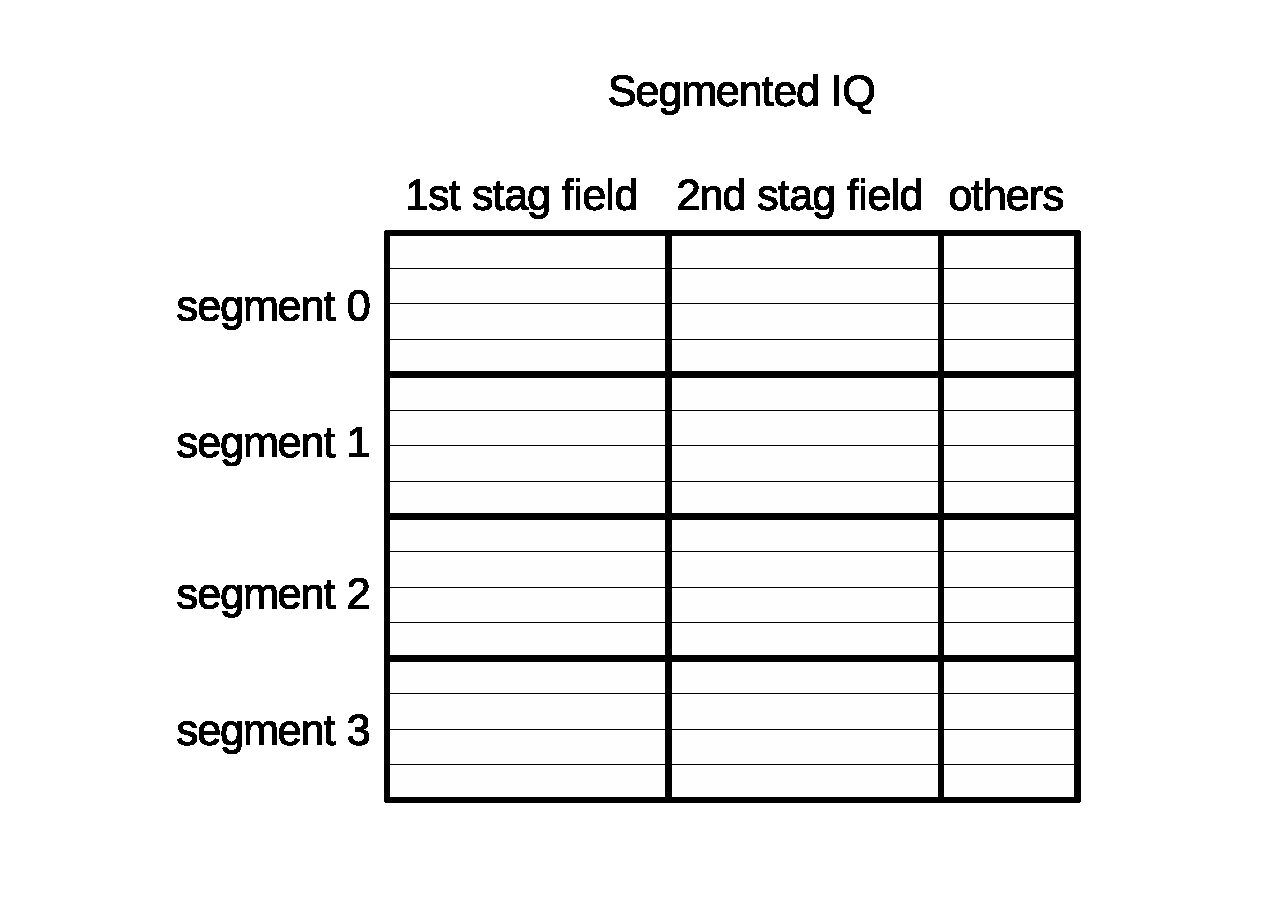
\includegraphics[keepaspectratio, scale=.8]{segmentedIQ}
  \caption{セグメント化した IQ}
  \label{fig:segmentedIQ}
\end{figure}

\subsection{提案手法の概要}
提案手法の基本アイデアは,大容量 CAM の電力削減に関する研究~\cite{Motomura1990paper, Motomura1990journal}から着想を得ている.この研究において提案されている手法では,CAM を複数の\textbf{セグメント}~\footnote{文献~\cite{Motomura1990paper, Motomura1990journal}ではバンクと呼ばれている.}に分割する.各セグメントには下位ビットが同一のデータのみを記録する.そして,タグ比較においては,比較対象のデータの下位ビットと,記録されているデータの下位ビットが一致するセグメントのみで比較を行う.これによって,比較器が動作する回数を「1/セグメント数」まで削減することができ,消費電力が削減できる.

本手法においても,\fig{segmentedIQ}に示すように IQ を複数のセグメントに分割する.各セグメントには,第 1 ソース・タグの下位ビットがセグメントの番号と一致する命令をディスパッチする.ウェイクアップ時の第 1 ソース・タグのタグ比較では,デスティネーション・タグの下位ビットとセグメントの番号が一致するセグメントのみでタグ比較を行う.これによって,第 1 ソース・タグのタグ比較回数を「1/セグメント数」に削減できる.

\subsection{提案手法におけるディスパッチ}
ディスパッチする IQ のエントリを決定する回路を\fig{dispatch}に示す.本手法では,フリー・リストをセグメントと同じ数だけ用意する.各フリー・リストは,対応するセグメントの空きエントリのインデクスを FIFO バッファで管理する.各フリー・リストからは IQ のインデクスが出力され,その中の1つを選択してディスパッチするエントリを決定する.どのフリー・リストからの出力を選択するかは,セグメント選択回路(図中の segment select logic)によって決定される.セグメント選択回路は,第 1 ソース・オペランドのタグ及びレディ・ビットと,各セグメントの空きエントリ数を入力とし,ディスパッチするセグメント番号を出力する.

セグメント選択回路の選択アルゴリズムについて説明する.セグメントの選択方法は,ディスパッチ時に第 1 ソース・オペランドがレディであるかによって異なるため,それぞれの場合に関して説明する.
\begin{itemize}
  \item \textbf{第 1 ソース・オペランドがレディでない場合}: 第 1 ソース・タグの下位ビットと番号が同じセグメントを選択する.選択されたセグメントに空きエントリがある場合,ディスパッチ可能であるため,対応するフリー・リストから読み出したエントリにディスパッチする.対応するセグメントに空きがない場合は,セグメントに空きが出るまでディスパッチをストールさせる.
  \item \textbf{第 1 ソース・オペランドがレディである場合}:この場合,第 1 ソース・タグの比較は行われないため,どのセグメントにディスパッチしても問題ない.このような場合を\textbf{セグメント・インディペンデント}と呼ぶ.この場合,空きエントリのあるセグメントから,ラウンドロビンでディスパッチするセグメントを選択しディスパッチする.
\end{itemize}
例として,第 1 ソース・オペランドがレディでなく,タグが 15(${\rm 1111_2}$)である命令を,\fig{segmentedIQ}に示す 4 つに分割された IQ にディスパッチする場合を考える.第 1 ソース・タグの下位 2 ビットが 3(${\rm 11_2}$)であるので,この命令は第 3 セグメントにディスパッチされる. 

なお,ソース・オペランドを使用しない命令も存在するが,そのような命令はディスパッチ時にソース・オペランドがレディであるものとして扱う.

\begin{figure}[htb]
  \centering
  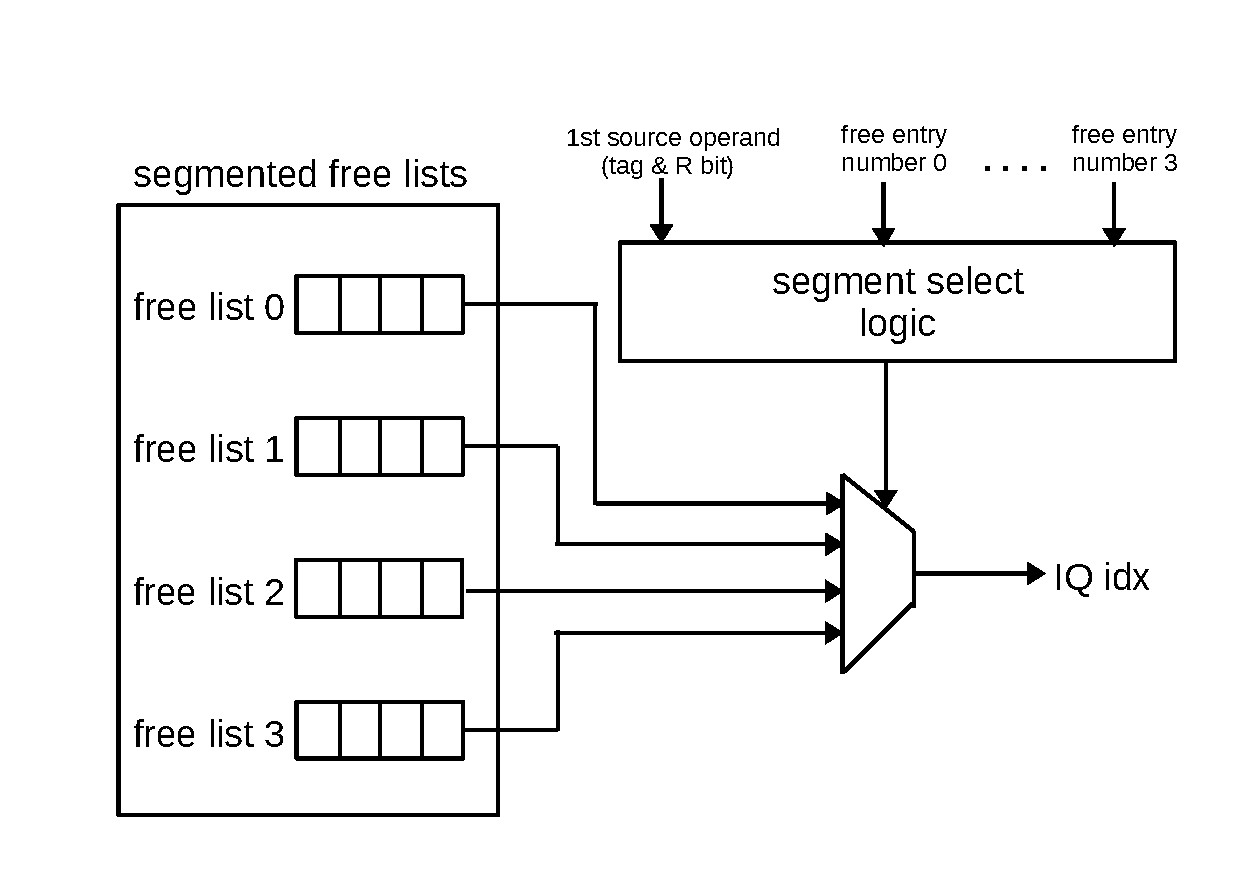
\includegraphics[keepaspectratio, scale=.8]{dispatch}
  \caption{提案手法におけるディスパッチエントリの決定回路}
  \label{fig:dispatch}
\end{figure}

\subsection{提案手法におけるウェイクアップ}
提案手法におけるウェイクアップでは,デスティネーション・タグの下位ビットがセグメント番号と一致するセグメントでのみ,第 1 ソース・タグのタグ比較器を動作させ比較を行う.一致しないセグメントはタグ比較器を動作させない.これは,デスティネーション・タグの下位ビットと番号が一致しないセグメントには,第 1 ソース・タグの下位ビットがデスティネーション・タグの下位ビットと異なる命令しか入っておらず,タグは必ず不一致となるためである.

例として,放送されたデスティネーション・タグが 6(${\rm 110_2}$)で,IQ が\fig{segmentedIQ}のように 4 つのセグメントに分割されている場合を考える.この場合,下位ビットは 2(${\rm 10_2}$)であるため,第 2 セグメントでのみ,第 1 ソース・タグのタグ比較を行う.

なお,第 2 ソース・タグのタグ比較に関しては,セグメントの番号とタグの下位ビットに関係性はないため,すべてのセグメントでタグ比較を行う必要がある.

提案手法におけるタグ比較の回路を\fig{segmentedIQ_wakeup}に示す.同図は 4 つのセグメントに分割された IQ のうち,第 0 セグメントのエントリにおける,第 1 ソース・タグの比較回路を示している.タグ・ビット数は 5 とし,発行幅を $IW$ とする.

タグ比較の動作を図中の番号を用いて説明する.\ctext{1}放送されるデスティネーション・タグの下位 2 ビットはデコーダ(SVSD:Segment-Validation Signal Decoder)へ送られる.SVSD はセグメント数だけ信号線を出力する.第 $n$ 番目の信号線は,第 $n$ セグメントでのタグ比較を有効化することを示す.つまり,デスティネーション・タグの下位ビットが $n$ の場合,$n$ 番目の出力線のみ $H$ を出力し,残りはすべて $L$ を出力する.SVSD の出力信号線のことを,以下, SVS(Segment-Validation Signal)と呼ぶ.

\ctext{2}AND ゲートによって,SVS が $H$ の場合にのみ,デスティネーション・タグの高位ビット及びその反転信号がタグ比較器へ入力される.\fig{segmentedIQ_wakeup}に示す回路は第 0 セグメントのタグ比較回路であるため,0 番目の SVS が AND ゲートに入力されている.

SVS が $H$ の場合,つまり,デスティネーション・タグの下位ビットとセグメント番号が一致していた場合のみ,比較器にデスティネーション・タグの高位ビットとその反転信号が送られ,ソース・タグの高位ビットと比較が行われる.SVS が $L$ の場合,デスティネーション・タグとその反転信号がどちらも $L$ としてタグ比較器へ入力される.この場合,デスティネーション・タグとその反転信号に接続されたプルダウン・トランジスタがすべて OFF となるため,マッチ線はディスチャージされず,電力を消費しない.

\ctext{3}タグ比較の結果,タグの高位ビットが一致した場合は,比較器から $H$ が出力される.

\ctext{4}タグ比較器が $H$ を出力し,かつ SVS が $H$ である場合に,タグ比較は一致となる.

\ctext{5}$IW$ 個の比較のいずれかが一致となった場合に,ソース・オペランドのレディ・ビットがセットされる.

SVSD の回路図を\fig{SVSD}に示す.SVSD はデスティネーション・タグの下位ビットのうち $log_2(セグメント数)$ ビットの正転及び反転信号を入力とし,セグメント数分の SVS を出力するバイナリ・デコード回路である.SVSD は セグメント数分の AND ゲートで構成される.

図ではセグメント数が 4 の場合の SVSD を表記しており,デスティネーション・タグの下位 2 ビット($log_2\:4$)を入力とし,SVS が 4 本出力される.赤字でタグの下位ビットが 2(${\rm 01_2}$)の場合を例示している.この場合,SVS2 のみ $H$ となり,その他の SVS は $L$ を出力する. 


\begin{figure}[thb]
  \centering
  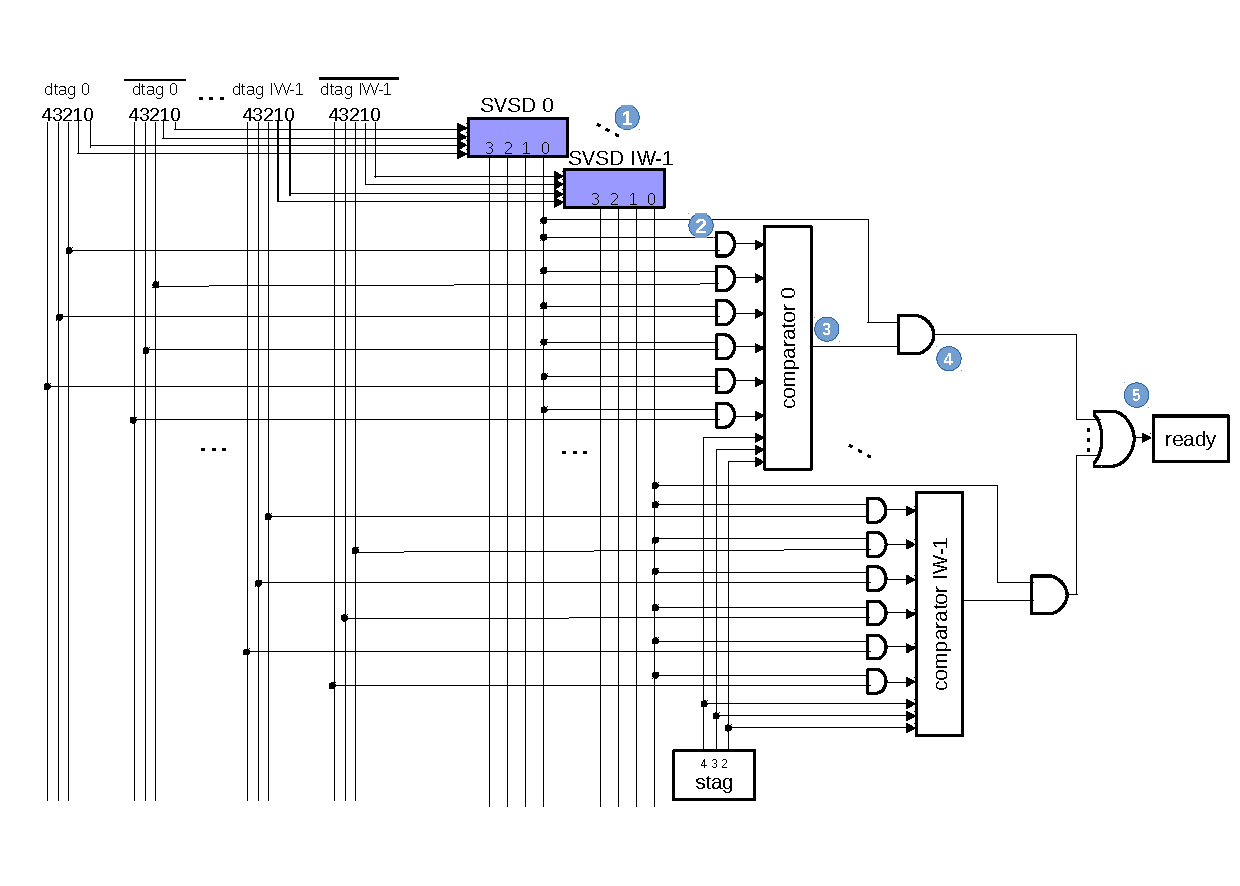
\includegraphics[keepaspectratio, scale=.8]{segmentedIQ_wakeup}
  \caption{提案手法におけるタグ比較回路(第 0 セグメント)}
  \label{fig:segmentedIQ_wakeup}
\end{figure}

\begin{figure}[htb]
  \centering
  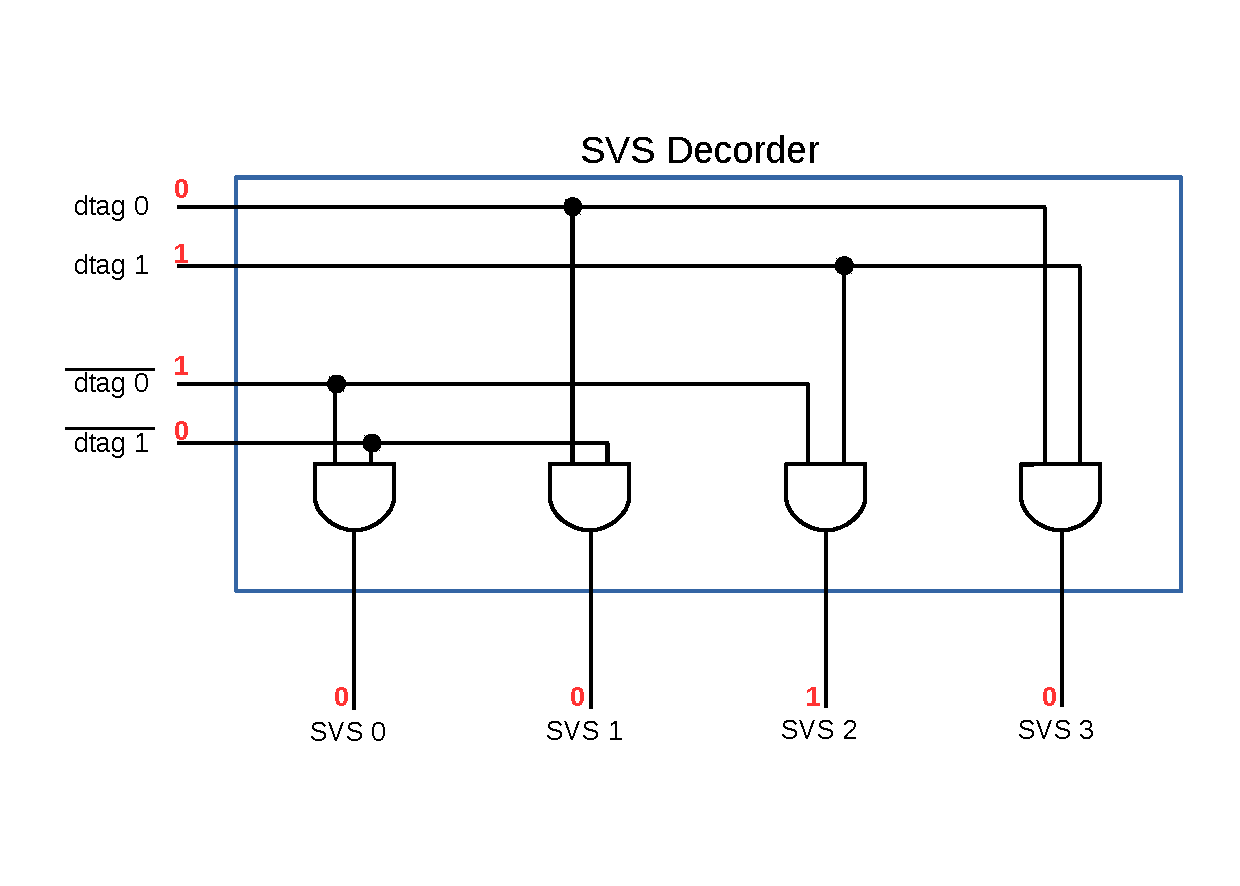
\includegraphics[keepaspectratio, scale=.8]{SVSD}
  \caption{SVSD(Segment-Validation Signal Decoder)}
  \label{fig:SVSD}
\end{figure}

% 図が後ろに行きすぎないように
\clearpage

%4 第 2 ソース・タグ比較の削減
\section{第 2 ソース・タグ比較の削減}
\label{sec:second_tag_comp}
\refsec{segmented_IQ}節で述べた手法では,命令の第 2 ソース・タグのタグ比較回数は削減できない.そこで本節では,第 2 ソース・タグの比較回数の削減を可能とする\textbf{スワップ}と\textbf{サブ・セグメント}という 2 つの手法を提案する.

\subsection{スワップ}
\label{sec:swap}
スワップは,第 1 ソース・タグと第 2 ソース・タグを格納するフィールドを交換し,第 2 ソース・タグの下位ビットをもとにディスパッチするセグメントを決定する手法である.以下で詳しく説明する.

第 1 ソース・オペランドがレディで,第 2 ソース・オペランドがレディでない場合について説明する.この場合,\refsec{segmented_IQ}で説明した方法では,命令はセグメント・インディペンデントとしてディスパッチされる.第 1 ソース・オペランドは既にレディであるため,比較は第 2 ソース・タグについてのみ行われるが,第 2  ソース・タグのタグ比較は全てのセグメントで行われるため,タグ比較の回数は削減されない.

そこでこのような場合に,第 1 ソース・タグと第 2 ソース・タグを交換し(スワップ),第 2 ソース・タグの下位ビットを使用してディスパッチするセグメントを選択する.これにより,\refsec{segmented_IQ}で述べたセグメント化の効果でタグ比較回数が削減される.なお,スワップではタグを交換するが,ペイロード RAM に格納するソース・タグを交換するわけではないので,命令の意味は保持される.

\subsubsection{スワップを行う場合のセグメント選択アルゴリズム}
セグメント選択回路は,\tab{agg_algorithm}に示すアルゴリズムによってディスパッチするセグメントを決定する.なお,表中のソース・タグの状態とは,ディスパッチ時にソース・オペランドがレディであるかどうかを示しており,(第 1 ソース・オペランド,第 2 ソース・オペランド)の形式で,R がレディであることを,NR がレディでないことを表す.

\begin{table}[htb]
  \caption{スワップを行う場合のセグメント選択アルゴリズム}
  \footnotesize
  \center
   \begin{tabular}{|l|l|} \hline \hline
    ソース・タグの状態 & アルゴリズム \\ \hline
    (NR,NR) & 第 1 ソース・タグでセグメントを選択する. \\ \hline
    (R,NR) & スワップを行い,第 2 ソース・タグでセグメントを選択する.\\ \hline
    (NR,R) & 第 1 ソース・タグでセグメントを選択する.\\ \hline
    (R,R) & セグメント・インディペンデントとしてラウンドロビンでセグメントを選択する. \\ \hline
  \end{tabular}
  \label{tab:agg_algorithm}
\end{table}
なお,両ソース・オペランドがレディのとき以外で,選択されたセグメントに空きがない場合は,ディスパッチをストールして当該のセグメントに空きが出るまで待ち合わせる.

\subsection{サブ・セグメント}
\label{sec:sub_segment}
サブ・セグメント方式は,第 1 ソース・タグの下位ビットに応じて分割されるセグメントを,第 2 ソース・タグの下位ビットに応じてさらに細かく分割する.第 2 ソース・タグの下位ビットによる分割をサブ・セグメント(S-seg)と呼び,従来の第 1 ソース・タグによる分割をサブ・セグメントに対応してメイン・セグメント(M-seg)と呼ぶこととする.

サブ・セグメントを導入した IQ の分割を\fig{sub_segment}に示す.黒色の枠で示す各メイン・セグメントを,赤色と青色で示すようにさらにサブ・セグメントに分割する.同図は,メイン・セグメント数が 4 ,サブ・セグメント数が 2 の場合の例を表しており, IQ は合計 $4 \times 2 = 8$ 個のセグメントに分割される.各セグメントの左には,(M-seg,S-seg)という形式でメイン及びサブ・セグメントの番号を表している.

サブ・セグメント方式について,ディスパッチとウェイクアップの動作をそれぞれ説明する.

\begin{figure}[htb]
  \centering
  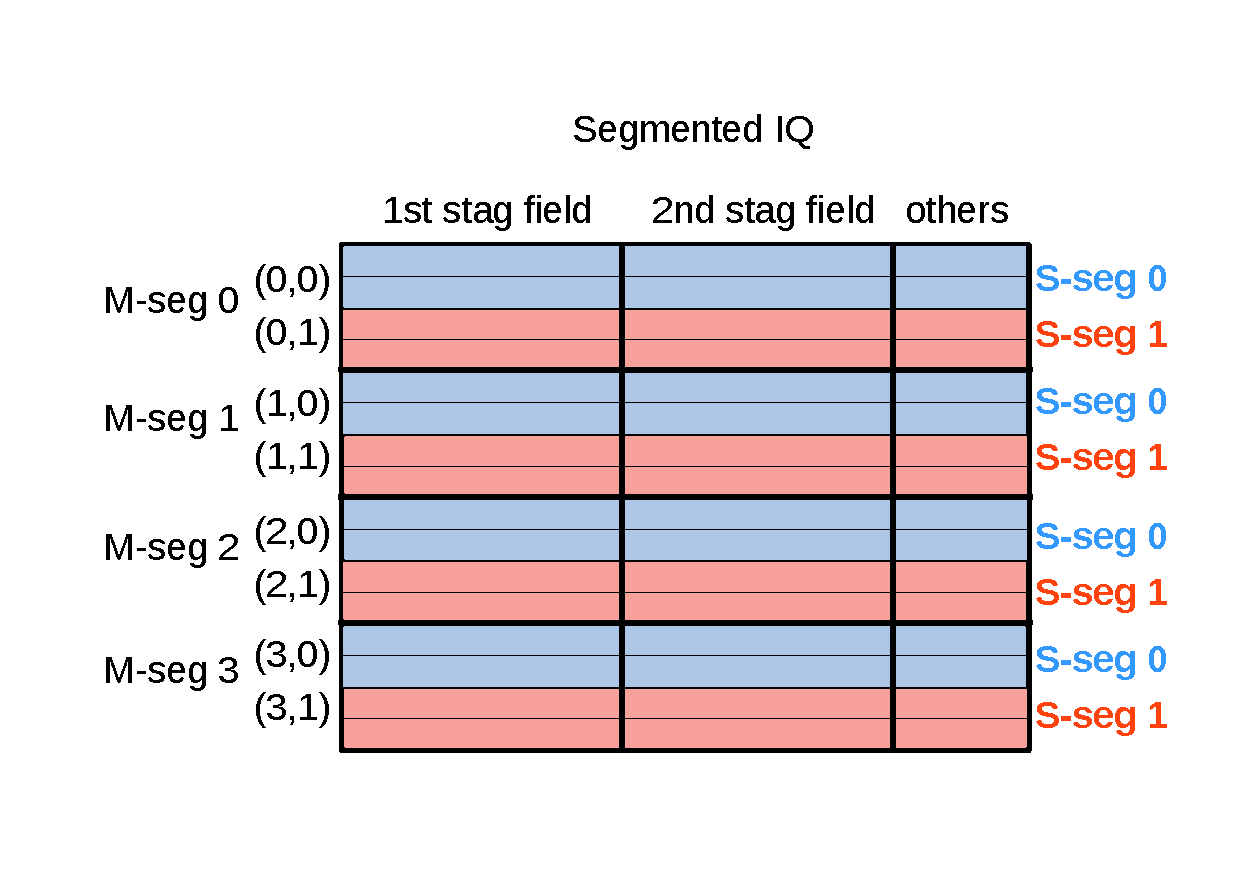
\includegraphics[keepaspectratio, scale=.8]{sub_segment}
  \caption{サブ・セグメントを実装した IQ}
  \label{fig:sub_segment}
\end{figure}

\subsubsection{サブ・セグメントにおけるディスパッチ}
サブ・セグメント方式におけるディスパッチにおいては,フリー・リストを M-seg $\times$ S-seg だけ用意する.\fig{sub_segment}に示した例の場合 8 個のフリー・リストが必要となる.

サブ・セグメント方式におけるセグメント選択のアルゴリズムに関して説明する.アルゴリズムはソース・オペランドのレディ状況によって異なるため,以下ですべての場合に関して説明する.説明を簡単にするため,命令 $p5 = p13 + p6$ を,\fig{sub_segment}に示す IQ にディスパッチする場合について例示する.第 1 ソース・タグが 13 で,第 2 ソース・タグが 6 である.
\begin{itemize}
  \item \textbf{両ソース・オペランドともレディでない場合}:第 1 ソース・タグでメイン・セグメントを,第 2 ソース・タグでサブ・セグメントを選択する.例の場合,第 1 ソース・タグ 13(${\rm 1101_2}$) の下位ビット 1(${\rm 01_2}$)より,メイン・セグメントは 1 となる.また,第 2 ソース・タグ 6(${\rm 110_2}$) の下位ビット 0(${\rm 0_2}$)より,サブ・セグメントは 0 となる.従って(1,0)のセグメントを選択する. 
  \item \textbf{第 1 ソース・オペランドのみレディである場合}:第 2 ソース・タグでサブ・セグメントを選択する.例の場合,第 2 ソース・タグ 6(${\rm 110_2}$) の下位ビット 0(${\rm 0_2}$)より,サブ・セグメントは 0 となる.第 1 ソース・オペランドは既にレディであるため,メイン・セグメントの制限はない.従って,(0,0),(1,0),(2,0),(3,0)のいずれかのセグメントをラウンドロビンで選択する.このように,メイン・セグメントの制限がない場合をメイン・セグメント・インディペンデント(M-seg インディペンデント)と呼ぶこととする.
  \item \textbf{第 2 ソース・オペランドのみレディである場合}:第 1 ソース・タグでメイン・セグメントを選択する.例の場合,第 1 ソース・タグ 13(${\rm 1101_2}$) の下位ビット 1(${\rm 01_2}$)より,メイン・セグメントは 1 となる.第 2 ソース・オペランドは既にレディであるため,サブ・セグメントの制限はない.従って,(1,0)または(1,1)のいずれかのセグメントをラウンドロビンで選択する.このように,サブ・セグメントの制限がない場合をサブ・セグメント・インディペンデント(S-seg インディペンデント)と呼ぶこととする.
  \item \textbf{両ソース・オペランドがレディである場合}:M-seg インディペンデントかつ S-seg インディペンデントであるため,空きのあるすべてのセグメントからラウンドロビンで選択する.
\end{itemize}

\subsubsection{サブ・セグメントにおけるウェイクアップ}
第 1 ソース・タグの比較は,デスティネーション・タグの下位ビットがメイン・セグメント番号と一致するセグメントのみで行う.また,第 2 ソース・タグの比較は,デスティネーション・タグの下位ビットがサブ・セグメント番号と一致するセグメントのみで行う.このような比較により,第 1 ソース・タグだけでなく,第 2  ソース・タグの比較に関しても,「1/サブ・セグメント数」まで削減が可能となる.

\subsubsection{サブ・セグメントとスワップの併用}
サブ・セグメント方式はスワップと併用することが可能である.併用する場合は,ディスパッチ時に第 1 ソース・オペランドのみレディである場合の選択アルゴリズムを,以下のように変更する.
\begin{itemize}
  \item \textbf{第 1 ソース・オペランドのみレディである場合}:スワップを行い,第 2 ソース・タグでメイン・セグメントを選択する.例の場合,第 2 ソース・タグ 6(${\rm 110_2}$) の下位ビット 2(${\rm 10_2}$)より,メイン・セグメントは 2 となる.第 1 ソース・オペランドは既にレディであるため,S-seg インディペンデントである.従って,(2,0)または(2,1)のいずれかのセグメントを選択する.
\end{itemize}
サブ・セグメント方式とスワップを併用することによって,ディスパッチ時に第 1 ソース・オペランドのみレディである命令におけるタグ比較回数の削減が「1/サブ・セグメント数」から「1/メイン・セグメント数」となる.従って,\fig{sub_segment}に示した分割のようにメイン・セグメント数がサブ・セグメント数よりも多い場合に,タグ比較回数をより多く削減できる.

サブ・セグメントとスワップを併用する場合のセグメントの選択アルゴリズムを\tab{agg_algorithm_subseg}にまとめる.

\begin{table}[htb]
  \caption{スワップを行う場合のセグメント選択アルゴリズム(サブ・セグメント併用)}
  \footnotesize
  \center
   \begin{tabular}{|c|p{13cm}|} \hline \hline
    ソース・タグの状態 & アルゴリズム \\ \hline
    (NR,NR) & 第 1 ソース・タグでメイン・セグメントを,第 2 ソース・タグでサブ・セグメントを選択. \\ \hline
    (R,NR) & スワップを行い,第 2 ソース・タグでメイン・セグメントを選択する.サブ・セグメントは S-seg インディペンデントとしてセグメントを選択.\\ \hline
    (NR,R) & 第 1 ソース・タグでメイン・セグメントを選択する.サブ・セグメントは S-seg インディペンデントとしてセグメントを選択.\\ \hline
    (R,R) & M-seg インディペンデントかつ S-seg インディペンデントとしてセグメントを選択. \\ \hline
  \end{tabular}
  \label{tab:agg_algorithm_subseg}
\end{table}

\section{提案手法におけるタグ比較回数の概算}
\label{sec:comp_estimate}
提案手法におけるタグ比較回数削減の効果を概算する.なお,サブ・セグメントを使用する場合も使用しない場合も,(R,NR)の場合にスワップを行うものとする.

概算するにあたり,次の 2 つの仮定をおく.
\begin{enumerate}
  \item 命令のソース・タグは 50\% の確率でディスパッチ時にレディであるとする.つまり,(NR,NR),(R,NR),(NR,R),(R,R) である命令の数は全て等しいとする.
  \item 提案手法による IQ の容量効率の低下(詳しくは\refsec{switch}で説明する)は全く生じないとする.
\end{enumerate}
上記の仮定をおいた場合に,提案手法を使用した場合のタグ比較回数は,以下の式で計算することができる(式の導出は\refapp{appendix1}で示す).

\[
  \frac{3}{4}\times\frac{1}{M\_seg} + \frac{1}{4}\times\frac{1}{S\_seg}
\]
ここで,$M\_seg$ はメイン・セグメント数を, $S\_seg$ はサブ・セグメント数を表す.なお,サブ・セグメントを使用しない場合は,$M\_seg$ をセグメント数とし,$S\_seg = 1 $ として計算すれば良い.

この式を用いて,本論文にて評価を行った全てのセグメント数の組み合わせにおける,タグ比較回数の概算を行った.その結果を\tab{comp_estimate}に示す.表に示しているタグ比較回数は,セグメント化しない通常の IQ に対する相対タグ比較回数を \% 形式で示している.

なお,以降の説明において,(メイン・セグメント数,サブ・セグメント数) の形式でセグメント数を表記する.また,サブ・セグメントを使用しない場合は,サブ・セグメント数は 1 と表記する.例えば,サブ・セグメントを使用せず,セグメント数を 16 とする場合は(16,1)と表記し,サブ・セグメントを使用し,メイン・セグメント数を 8 ,サブ・セグメント数を 2 とする場合(8,2)と表記する.

\begin{table}[htb]
  \caption{タグ比較回数の概算}
  \footnotesize
  \center
    \begin{tabular}{c|c|c} \hline \hline
    総セグメント数 & (M-seg,S-seg) & 相対タグ比較回数(\%) \\ \hline
    4 &(4,1) & 44 \\
    &(2,2) & 50 \\ \hline
    8 &(8,1) & 34 \\
    &(4,2) & 31 \\ \hline
    &(16,1) & 30 \\
    16 &(8,2) & 22 \\
    &(4,4) & 25 \\ \hline
    &(32,1) & 27 \\
    32 &(16,2) & 17 \\
    &(8,4) & 16 \\ \hline
  \end{tabular}
  \label{tab:comp_estimate}
\end{table}

表より,総セグメント数が多くなるほど,タグ比較回数が少なくなることがわかる.また,総セグメント数が同じ場合,総セグメント数が 4 の場合を除いて,サブ・セグメントを使用する方がタグ比較回数が少ないことがわかる.これは,サブ・セグメントを用いることによって,(NR,NR)の場合に第 2 ソース・タグの比較回数が削減できるようになる効果が大きいためである.

なお,実際のタグ比較回数は,\refsec{switch}で説明する IQ の容量効率の低下により,計算した概算値よりも少なくなる.

% 
\chapter{まとめ}
\label{sec:summary}
LSIの微細化の進展に伴って,経年劣化が加速し摩耗故障が増加する問題が深刻になっている.この故障は,デバイスの温度に関して指数関数的に加速するため,チップ内のホット・スポットの解消が求められている.

発行キューはこのホット・スポットの 1 つとして知られている.この主な原因はウェイクアップ時の多数のタグ比較である.本論文では,ウェイクアップ時のタグ比較回数を削減するために,発行キューをセグメント化する方法を提案した.また,提案手法におけるタグ比較削減の効果を高める手法であるスワップとサブ・セグメント及び,提案手法によって生じる性能低下を抑制する手法である SWITCH 方式を合わせて提案した.

提案手法を SPEC CPU 2017 を使って評価したところ,性能低下を最大でも 5\% 以下に抑えつつ,タグ比較回数を 82\% 削減できることを確認した.



% 付録(必要に応じてコメントを外したり,新たに追加する)
% \appendix
% 
\chapter{提案手法のその他の工夫}
\label{sec:appendix1}
提案手法によるタグ比較回数をより減らすための工夫として,Last Tag Prediction(LTP) という手法が有効ではないかと考え,シミュレータに実装し評価を行った.本章では,LTP とその評価結果に関して説明する.なお,評価の結果,LTP はあまり効果がないことがわかったため,最終的な提案手法には実装していない.

\section{LTP:Last Tag Prediction}
CONSARVARTIVE 方式 において,第 1 ソース・タグと第 2 ソース・タグがどちらもレディでない命令は,以下のアルゴリズムでセグメントを選択すると述べた.

\begin{itemize}
  \item サブ・セグメントを使用しない場合:第 1 ソース・タグでセグメントを選択する.選択したセグメントに空きがない場合,スワップして第 2 ソース・タグをもとにセグメントを決定する.なおも空きがない場合はストールする.
  \item サブ・セグメントを使用する場合:第 1 ソース・タグでメイン・セグメントを,第 2 ソース・タグでサブ・セグメントを選択する.選択したセグメントに空きがない場合,スワップを行い,第 2 ソース・タグでメイン・セグメントを,第 1 ソース・タグでサブ・セグメントを選択する.スワップしてなおも空きがない場合はストールする.
\end{itemize}

このアルゴリズムにおいて,スワップする場合としない場合に選択されるセグメントのどちらにも空きがある場合を考える.このような場合,CONSERVATIVE のアルゴリズムでは,スワップを行わずにディスパッチするセグメントを決定する.

このような場合に,レディとなるのがより遅く,比較がより多く行われるソース・オペランドのタグ(ラスト・タグ)を第 1 ソース・タグのフィールドに書き込むようにセグメントを選択すれば,タグ比較回数をより多く削減できると考えられる.ただし,ラスト・タグがどちらになるかという情報はデコード時にはわからないため,予測を行う必要がある.

ラスト・タグの予測方法は,論文~\cite{ernst2002}で提案されている.この方法を Last Tag Prediction(LTP)と呼ぶ.以下,LTP による予測とセグメントの選択方法に関して説明する.

\begin{figure}[htb]
  \centering
  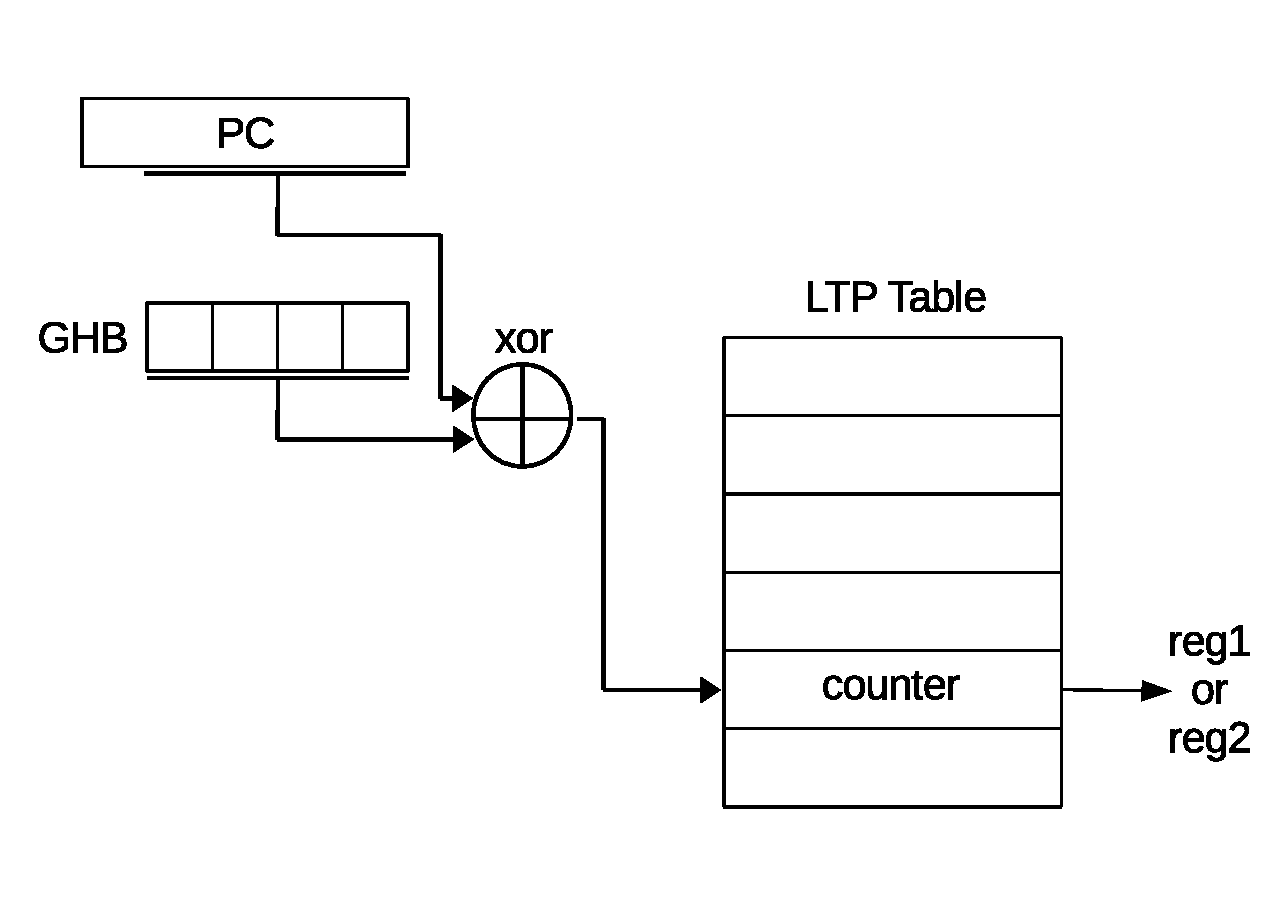
\includegraphics[keepaspectratio, scale=.8]{ltp}
  \caption{LTP の構成}
  \label{fig:ltp}
\end{figure}

LTP は,\fig{ltp}のように.命令の PC の下位ビットビットとグローバル分岐履歴(GHB:Global History Buffer)のハッシュをインデクスとするテーブル(LTP Table)で構成される.LTP Table の各エントリは 2 ビットの飽和型アップ・ダウン・カウンタで構成され,このカウンタは,値が 0 または 1 の場合に第 1 ソース・タグがラスト・タグであることを示し, 2 または 3 の場合に第 2 ソース・タグがラスト・タグであることを示す.予測と学習の方法について説明する.
  
\subsection{予測方法}
命令ディスパッチ時に,第 1 ソース・タグと第 2 ソース・タグがともにレディでなく,なおかつスワップした場合としない場合に選択されるセグメントがいずれもディスパッチ可能な場合に予測が行われる.予測の際には,PC と GHB のハッシュを用いてテーブルを検索し,該当するエントリのカウンタ値を読み出す.

第 1 ソース・タグがラスト・タグであると予測された場合には,スワップを行なわずにセグメントを選択しディスパッチする.第 2 ソース・タグがラスト・タグであると予測された場合には,スワップを行いセグメントを選択し,ディスパッチする.
  

\subsection{学習方法}
学習は命令発行時に,ディスパッチ時に予測を行った命令でのみ行われる.命令発行時に,第 1 ソース・タグと第 2 ソース・タグがレディとなったサイクルを比較する.第 1 ソース・タグ のほうが遅かった場合にはカウンタをデクリメントし,第 2 ソース・タグのほうが遅かった場合にはカウンタをインクリメントする.

\section{LTP の評価}

% 発表実績(なければコメントアウトしておく)

\chapter*{発表実績}
\addcontentsline{toc}{chapter}{発表実績}
\begin{itemize}
  \item 森健一郎, 安藤秀樹, ``容量効率を意識したソース・タグ値に基づくセグメント化による発行キューのエネルギー削減'', 情報処理学会研究報告, Vol.2020-ARC-241, No.3, pp.1-12, 2020年7月
\end{itemize}

% 謝辞

\chapter*{謝辞}
\addcontentsline{toc}{chapter}{謝辞}
本研究を進めるにあたり,多大なる御指導と御鞭撻を賜わりました名古屋大学大学院工学研究科 情報・通信工学専攻 安藤秀樹教授に心より感謝いたします.また,本研究の遂行を支えてくださいました,名古屋大学大学院工学研究科情報・通信工学専攻安藤研究室の諸氏に深く感謝します.

% ---------- ユーザ入力ここまで ----------


% 参考文献
\bibliographystyle{IEEEtran} 
\bibliography{ref_swopp}

\end{document}
